\section{Algorithmic investigations}
\label{sec:algo}

The investigations follow the inverse problem of Figure~\ref{fig:map}, from the
observation to the search, the constraints and the supervision. Each starts from
the property of the problem that motivates a mechanism, then gives its
formulation and implementation, the experiment that isolates it, and what the
outcome says about the system.

\subsection{Mesh conditioning and skeleton-aware part assignment}
\label{sec:prep}

\textbf{Motivation.} The objective observes only the scan surface, so defects in
that surface are defects in the observation: holes, disconnected fragments,
non-manifold edges and debris, and thin appendages that vanish under naive
simplification (Figure~\ref{fig:raw-scans}). The question is whether repairing the
observation is the lever on registration accuracy (RQ1).

\textbf{Mechanism.} Two repair strategies are complementary. Alpha Wrap~\cite{alphawrap} shrink-wraps the input: a
facet is traversable only if its circumradius exceeds $\alpha$, so cavities and
holes smaller than $\alpha$ stay closed, while the offset sets the distance of the
output from the input; the result is watertight, 2-manifold, intersection-free and
strictly enclosing even for defective input, and a smaller $\alpha$ penetrates
deeper into concavities at the cost of reproducing more of the defects. The
trade-off is therefore set by $\alpha$ relative to the thinnest structure to
preserve, with the offset kept a small fraction of it.
ManifoldPlus~\cite{manifoldplus} instead extracts the exterior faces between
occupied and empty voxels and projects the result back onto the input without
relying on face normals, and can recover zero-volume structures; it serves where
the wrap does not preserve thin parts. Every wrapped mesh passes a fidelity gate on
its worst deviation from the input, and topology-preserving quadric-error
reduction~\cite{qem} completes the stage. On a 50-specimen benchmark every output
was watertight (against none of the inputs) and most were a single connected
component; the fallback was needed on a quarter of the specimens.



\textbf{Evaluation design and finding.} Holding registration fixed, the fit on
cleaned meshes was compared with the fit on raw meshes, and each was scored
\emph{twice}, against the cleaned and against the raw target, so that an easier
scoring target could not be mistaken for a better registration. The sign flips:
cleaning looks like a gain of several per cent against the cleaned target, a loss
against the raw target, and the target-independent metrics show marginally more
distortion after cleaning. Mesh conditioning improves topology and the scoring
target without improving the registration, so input quality is a precondition for
fitting and not the factor that decides anatomical accuracy. The work was
redirected on this basis.

\textbf{Skeleton-aware part assignment.} Several downstream analyses require
deciding which structure a surface point belongs to. Assigning each point to the
nearest coxa anchor starves the middle legs, because a middle-leg point can sit
closer to a neighbouring anchor than to its own. Assigning instead to the nearest
\emph{articulated bone segment}, the standard primitive in skeletal rigging,
treats each leg as the connected chain it is, and raised the macro-averaged F1 of
the part labelling on the template from $0.66$ to $0.83$, with the largest gain at
the middle legs. The model priors of Section~\ref{sec:objective} (joint limits,
bilateral symmetry, the scale barrier) act on the same principle but constrain
\emph{plausibility}: they remove impossible configurations without selecting the
correct one. A Gaussian shape prior added as a stabiliser was removed once it was
found to suppress genuine morphological variation, which is the signal the model
exists to preserve.

\subsection{The Shape Diameter Function as structural information}
\label{sec:sdf}

If identity cannot come from the data term, a pose-independent intrinsic
descriptor might supply coarse anatomical structure before dense correspondence is
resolved. The Shape Diameter Function (SDF)~\cite{sdf}, a scalar measure of local
thickness obtained from rays cast into the solid behind each surface point, is
computable on a raw scan, independent of pose, and small on thin structures. It
separates body from appendage reliably (AUC $\approx0.97$) and is reproducible
across real scans (correlation $0.77$--$0.94$). Instance separation additionally
requires information that distinguishes repeated structures: on real scans the two
mandibles fell into one connected component in $9$ of $12$ specimens, because
connected components cannot split structures that are physically fused and local
thickness does not encode laterality.

This is an instance of a known limitation of intrinsic descriptors: when a shape
has an orientation-reversing self-symmetry, a loss that depends only on intrinsic
quantities has at least two equally valid optima, which is why orientation-aware
formulations were developed~\cite{donati}. The SDF therefore provides class-level
structure (which kind of part) and leaves instance-level identity (which side,
which leg) to be supplied by another source.

\subsection{Learned pose initialisation}
\label{sec:pointnet}

\textbf{Motivation.} The registration objective is non-convex, and its
nearest-surface assignments depend strongly on the initial articulated state. A
fixed canonical pose therefore determines which target regions become the
optimiser's initial attractors, so a poor start commits each leg to the wrong
basin before refinement begins. This motivates an input-conditioned initialiser,
which does not replace optimisation but changes the starting point from which the
non-convex latent space is explored.

\textbf{Formulation and implementation.} The initialiser regresses the initial
rotations of the leg joints from the scan, after which the differentiable fitter
performs local refinement (Figure~\ref{fig:pointnet}). The scan is first
canonicalised using the body-core vertices only, since a frame computed from the
full cloud lets leg pose leak into the reference frame meant to be
pose-invariant. Each of 2048 points carries its canonical coordinates and a
one-hot leg-chain identifier, and the sample is balanced between leg and body
points. A PointNet-style encoder~\cite{pointnet} applies a shared pointwise MLP
and aggregates with max pooling, a symmetric function that makes the descriptor
invariant to point ordering, which a raw scan does not have; a fully connected head
then predicts a continuous 6D rotation representation~\cite{zhou6d} per leg joint,
converted to a rotation matrix by Gram--Schmidt orthogonalisation and trained with
the same geodesic loss used for evaluation, on a 5000-specimen synthetic corpus
generated from the model.

\begin{figure}[!htb]
\centering
\begin{tikzpicture}[every node/.style={font=\footnotesize},
 box/.style={draw,rounded corners=2pt,minimum height=9mm,align=center,fill=white,inner sep=2pt},
 arr/.style={-{Stealth[length=1.6mm]}}]
\node[box] (a) {scan points\\body-core\\canonicalised\\$N\times(3{+}K)$};
\node[box,right=4.5mm of a] (b) {shared\\pointwise\\MLP};
\node[box,right=4.5mm of b] (c) {symmetric\\max-pool};
\node[box,right=4.5mm of c] (d) {global\\descriptor};
\node[box,right=4.5mm of d] (e) {MLP head\\6D rotation\\per leg joint};
\node[box,right=4.5mm of e,fill=blue!10] (f) {$\bm\theta_0$\\differentiable\\fitter};
\foreach \x/\y in {a/b,b/c,c/d,d/e,e/f}{\draw[arr] (\x)--(\y);}
\end{tikzpicture}
\caption[Learned pose initialiser]{Learned pose initialiser. Max pooling makes the
global descriptor invariant to point ordering; the predicted initial leg rotations
seed the differentiable fitter, which performs local refinement.}
\label{fig:pointnet}
\end{figure}

\textbf{Where an initial error does its damage.} Starting from the ground-truth
pose instead of the default repairs the thin distal structures (the pretarsus
error falls about twelvefold) and leaves the proximal attachment unchanged
(Figure~\ref{fig:init-sensitivity}, left). A matched experiment that fixes the total
pose error and varies only its position along the kinematic chain isolates the
reason (right): the same error is recoverable at the tip and damaging at the base,
because a proximal mistake propagates through every joint downstream. At proximal
attachment joints, pose interacts with scale and shape: several latent variables
jointly determine the same surface location, so correct pose alone does not fix it.
The fitter drifts from the pose it is seeded with in every segment, and the error
at the coxa, the clearest instance, correlates with the error in the per-joint
scales and not with pose drift. On exact synthetic meshes the coxa also carries a
label-ambiguity floor from neighbouring coxae, which must be read through.

\begin{figure}[!htb]
\centering
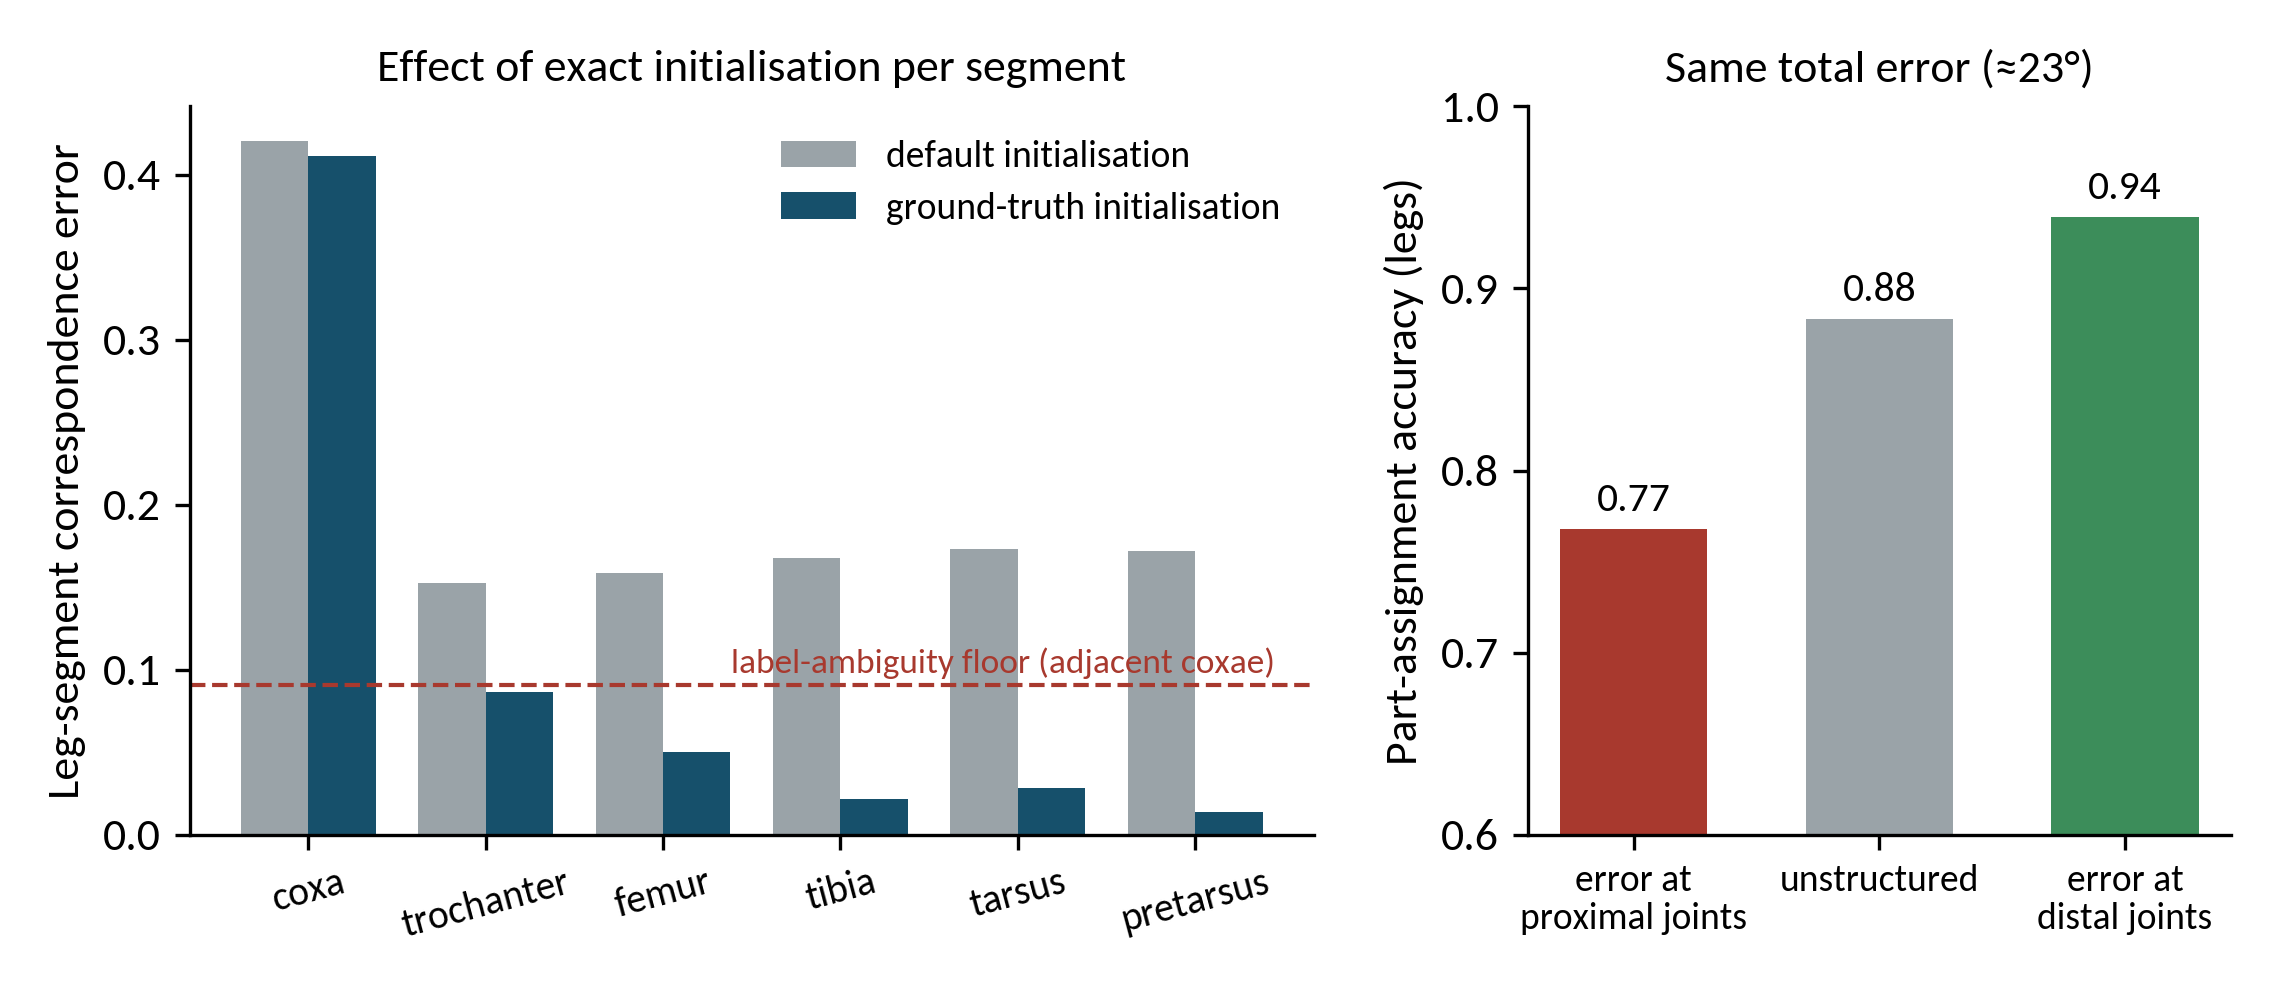
\includegraphics[width=0.74\linewidth]{figures/fig_init_sensitivity.png}
\caption[Sensitivity to initialisation]{Left: per-segment correspondence error under
default and ground-truth initialisation (synthetic, $n=48$); the dashed line is the
label-ambiguity floor at neighbouring coxae. Right: part-assignment accuracy for the
same total pose error ($\approx23^{\circ}$) placed at proximal joints, unstructured, or at
distal joints (synthetic, one seed per condition).}
\label{fig:init-sensitivity}
\end{figure}

\textbf{Transfer.} The learned initialiser improved controlled synthetic recovery
across all metric families. On 50 real specimens, trained at the synthetic
perturbation magnitude, it was significantly worse than the default, and a
controlled sweep of that magnitude moved it monotonically to parity. This separates
the value of input-conditioned initialisation from the question of
synthetic-to-real generalisation: the operative factor is the training
distribution, and the remedy lies there and not in the architecture. The same
sensitivity appears in the expert benchmark, where learned initialisation is
neutral on most specimens and decisive, in the wrong direction, on a few.

\subsection{Sampling and robust optimisation}
\label{sec:sampling}

The surface term is a Monte Carlo estimate,
$\mathcal L_{\mathrm{ch}}\approx\mathbb E_{x\sim p(x)}\big[\operatorname{dist}(x,T)^2\big]$, so the sampling
distribution $p(x)$ determines which anatomical regions contribute most to the
gradient. With $p$ proportional to surface area, the body and head dominate and
thin distal structures are severely under-represented in the optimisation measure.
The template makes this concrete: by dominant skinning weight, one leg has
$200$--$275$ vertices at the coxa and trochanter, $38$ at the tarsus and $8$ at the
pretarsus. Reserving a sampling quota for distal points improved the legs but
starved the antennae and head, which shared the budget; starvation is a real
confound, and controlling it does not by itself create anatomical correspondence.

Robust optimisation addresses points that are simply wrong. Graduated
non-convexity (GNC)~\cite{gnc} starts from a convex surrogate and progressively
hardens a robust cost, needs no initial guess and tolerates large outlier fractions,
without a global-optimality guarantee. Restricted to the leg points it improved
scores under synthetic corruption, whereas applied to the whole body it distorted
the antennae; its effect on clean data was not reproduced under a paired bootstrap,
and the metric behind the early corruption result has since been redefined. GNC is
carried as an additional robustness direction with a defined verification protocol,
not as a component of the shipped recipe.

\subsection{Physical plausibility: inter-part penetration}
\label{sec:penetration}

\textbf{Motivation.} Neither the surface term nor the model priors prevent one part
from passing through another: a leg that crosses the abdomen is a perfectly
reasonable surface to a Chamfer term. Articulated body-model fitting has long
included an interpenetration term for this reason~\cite{bogo}, and a penalty on
inter-part penetration, with an inside/outside decision from nearest-triangle
proximity, was added to the objective.

\textbf{Finding.} On 50 specimens the penalty made contact shallower (mean
penetration depth fell by about $40\%$) without reducing how often collisions
occur (the number of penetrating instances rose by about $17\%$, improving on 23
specimens and worsening on 27), and it degraded surface fit by more than $3\%$ on a
third of specimens. A chain of pre-registered hypotheses localised the mechanism.
That pose is held fixed while the penalty acts was falsified, since the rotations
were in fact used; a clamp on the loss contribution was excluded; and releasing the
smoothness terms that could drag neighbouring vertices into contact gave no
improvement under a causal intervention. Two mechanisms were confirmed: the
asymmetric density of the Chamfer samples across the two parts of a pair, and the
accuracy of the proximity-based inside/outside test, which disagrees with the
generalised winding number~\cite{jacobson} precisely in the direction of the pair
that fails to improve.

\textbf{Implication.} A plausibility constraint is only as reliable as its
inside/outside test and its sampling, and it must be evaluated on both the count and
the depth of violations, since depth alone can improve while the failure persists.
The evidence-supported next step is a winding-number-based test as the loss's core
signal, which was not part of the investigation.

\subsection{Learned dense correspondence}
\label{sec:learned-correspondence}

\textbf{Motivation and formal distinction.} A learned descriptor $f$ supports
\emph{retrieval}, $j^\ast(i)=\arg\min_j\|f(q_i)-f(t_j)\|$, a relation that places no
constraint on coverage or consistency. A dense \emph{correspondence}
$\pi:\mathcal S_A\rightarrow\mathcal S_B$ additionally requires global consistency,
coverage and structural coherence, which is why the correspondence literature
treats local descriptors and globally consistent maps separately, from functional
maps~\cite{fmaps} to embedding formulations~\cite{cse,haugaard} and recent
surveys of the field~\cite{survey}. In optimal-transport form, a coupling $P$ with
prescribed marginals,
$\min_{P\in\Pi(\mu,\nu)}\langle P,C\rangle-\varepsilon H(P)$~\cite{ot}, is what
enforces coverage, and unbalanced variants accommodate incomplete scans.

\textbf{Training logic.} The descriptor shares the backbone and warm start of an
existing contextual embedding (a PointNet++-style network trained with an InfoNCE
objective on exact vertex identity), but is trained for the task actually
evaluated. For a pair of specimens $(A,B)$ and a part, the positive for vertex $i$ is
vertex $i$ on $B$, and the negatives are all other vertices \emph{of the same part}
on $B$: the evaluation task is the loss, and the negatives are within-part by
construction. The input is raw posed coordinates, because normalising away a part's
length and radius removes information that carries correspondence signal. All arms
use one fixed sampling density at training and evaluation (4096 vertices), since the
backbone is out of distribution at five times its training density, with disjoint
training and held-out specimens asserted at run time. Candidates are restricted to
the same part, and the baseline is Euclidean nearest-neighbour matching computed on
exactly the same subsets.

\textbf{Finding.} The learned descriptor beats the Euclidean baseline at the coxa,
where raw proximity is least informative, and the gain strengthens with training; the
other segments do not clear the bar (Figure~\ref{fig:local-vs-dense}a). Pairwise
retrieval accuracy at one joint is thus evidence that learning captures information
raw geometry does not. Deployed in the form the fitter consumes (a target array over
all template vertices), the same descriptor is worse on every one of 48 specimens
than template-embedding lookup in the style of continuous surface
embeddings~\cite{cse}, and its votes collapse onto few template vertices
(Figure~\ref{fig:local-vs-dense}b,c). Restricting the baseline to the descriptor's own
candidate set changes the result by only a few per cent, so the gap is not an
artefact of the comparison. The descriptor is a query-to-query matcher with no
template embedding, so identity of the template has to be carried by reference
specimens; a mechanism that couples the votes into one consistent assignment is what
is missing. This is the benchmark-versus-system gap that evaluation work calls
external validity~\cite{liao}.

\begin{figure}[!htb]
\centering
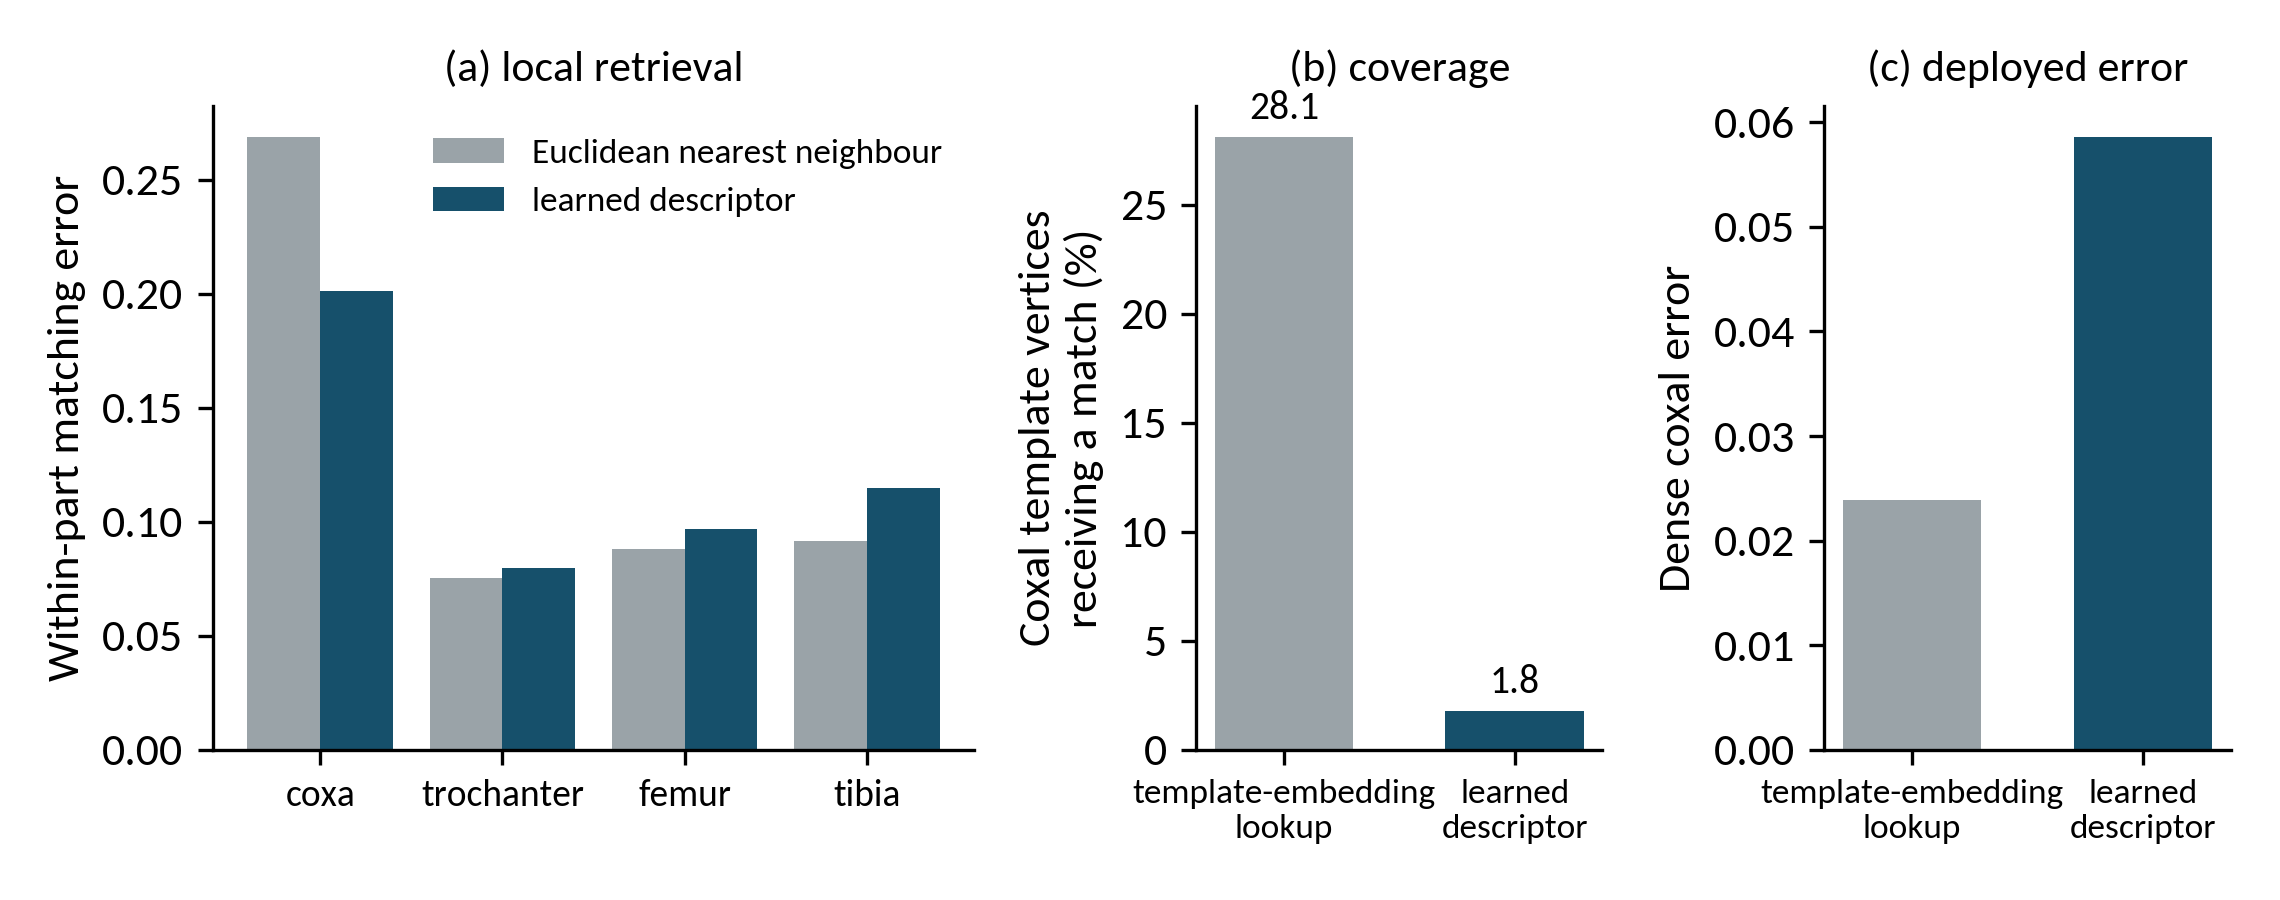
\includegraphics[width=0.70\linewidth]{figures/fig_local_vs_dense.png}
\caption[Local retrieval versus dense assignment]{The same descriptor at two levels.
(a) Within-part matching error against the Euclidean nearest-neighbour baseline: the
learned descriptor wins at the coxa. (b) Fraction of coxal template vertices that
receive a match and (c) dense coxal error when the descriptor is deployed as a full
assignment: strong local retrieval does not imply a usable dense correspondence.}
\label{fig:local-vs-dense}
\end{figure}

A linear probe of the network's features recovers the circumferential angle on tubular
segments far better than chance although retrieval on the same features is poor: the
information is present in the representation and the contrastive objective does not exploit
it, in line with the expectation that correspondence distributions become multi-modal on
symmetric surfaces~\cite{haugaard}. The within-part descriptor above is a query-to-query
matcher with no template embedding, which is exactly what the next subsection adds.

\subsection{A template-embedding head and the location of the residual}
\label{sec:cse}

\textbf{Design.} Every template vertex receives a learned key, and a scan point is matched to the
nearest key~\cite{cse}, so the output is a map over the whole template and not a set of local
votes. The head sits on a hierarchical point-set backbone~\cite{pointnet2} and emits a unit-norm
query per point, trained with a contrastive query--key (InfoNCE) loss on exact vertex identity,
the form that keeps symmetric regions from collapsing to an average~\cite{haugaard}; retrieval is
then a nearest-neighbour search in the embedding, which tolerates noise and partial scans~\cite{coe}.
No hand-designed coordinate system is involved. Each step was gated by a bar fixed before the run.

\textbf{What it established.} A frozen backbone already carried cross-specimen identity, strongly
along a limb and weakly around it, the failure expected of a deterministic embedding on a tubular
part; the contrastive key table improved the
circumferential component by a factor of two to four, the outcome predicted before the head was
written. Two design decisions proved decisive. \emph{How predictions reach the fitter:} given
as direct vertex identity they exceeded exact labels passed through a centroid and
inverse-kinematics conversion, which discards a large share of the achievable gain, so the
mechanism of consumption matters as much as accuracy. \emph{Which predictions to trust without
ground truth:} embedding similarity is entangled with ambiguity, as a point in a confusable
region scores high because it is confusable (the same pathology seen in learned feature
matching~\cite{lightglue}), whereas a cycle-consistency test (scan
point to vertex and back) is structural and, unlike similarity, lowers retrieval error when
used as a filter; it needs no ground truth and no segment whitelist. Deployed this way, the
term improved both part-level and leg-level accuracy on an independent synthetic corpus, and the
fit on nearly every real specimen. Retrieval quality and fitter sensitivity are only loosely coupled, so each gain was tested at the
fitter, and a small-sample estimate was corrected by an independent replication.

\textbf{Where the remaining error lives.} Stratified against a paired ceiling (the ground-truth
mesh scored as the fit), the residual is proximal: the coxa and trochanter own most of it and
the distal segments, which absorbed most of the investigation, own very little. The coxa is not a
correspondence problem: it is fitted as accurately as the body, and its apparent failure comes from
the fitter's general precision coinciding with the spacing between adjacent coxae, which makes a
nearest-vertex metric maximally sensitive there; reweighting the dense term by inverse tolerance
leaves it unchanged. The only intervention that moved it removed free deformation and paid for it in
shape accuracy: the pose--deformation trade-off of Section~\ref{sec:identifiability},
observed at one joint.

\textbf{Hypotheses ruled out.} Table~\ref{tab:closed} lists plausible and costly directions that
were tested against pre-registered bars and rejected; they are as informative as the positive
results.

\begin{table}[!htb]
\centering
\caption{Hypotheses tested against pre-registered bars and rejected.}
\label{tab:closed}
\small
\begin{tabular}{@{}L{0.37\linewidth}L{0.55\linewidth}@{}}
\toprule
\textbf{Hypothesis} & \textbf{Outcome}\\
\midrule
Circumferential signal is absent, so an equivariant network is needed & Present in the features and
 the geometry; the deficit is in the objective\\
Harder same-segment negatives surface it & Overall retrieval improved, the targeted component did not\\
Selecting among several candidates reaches the oracle headroom & Learned ranking and
 optimal-transport assignment~\cite{ot} each captured a small fraction\\
Softer targets or more embedding capacity help & Neither; the keys are not capacity-limited\\
The coxal error is a pose error, a single registration term, or a weighting problem & None of
 these; seeding, ablations and tolerance weighting leave it unchanged\\
\bottomrule
\end{tabular}
\end{table}

\subsection{Objective identifiability, deformation and staged optimisation}
\label{sec:identifiability}

The pose--deformation ambiguity of Section~\ref{sec:objective} predicts a specific
failure: free deformation is an escape hatch. A wrongly posed joint can be repaired
either by rotating it to the right angle or by bending the mesh around the wrong
angle until the surface term is satisfied; the two solutions are nearly
indistinguishable by Chamfer and anatomically unrelated, and only the first preserves
the correspondence needed for measurement (Figure~\ref{fig:gauge}). Neither an unbounded nor a frozen deformation budget is correct, so the
deformation cost acts as a regulariser whose weight sets the conditioning of the
pose; in the earlier synthetic round-trip study, raising that weight was the single most
effective change for correspondence accuracy.

Optimisation dynamics can silently remove part of the latent space. In the
hierarchical schedule the ratio of the pose and shape learning rates left the shape
vector almost fixed (its spread across specimens two to three orders of magnitude
smaller than in the unconstrained schedule), an effect invisible to every surface
metric and found only through a latent-space diagnostic. A second instance came from
the fitting schedule: pose was held fixed for $2000$ of the $2400$ refinement
iterations, so a pose error could only be absorbed by denting the mesh, and the
Chamfer curve descended smoothly regardless; a widened pose-adjustable window
improved nearly every integrity metric at no cost and was adopted.

A third instance concerns priors that carry no anatomical content. The per-joint scale
barrier introduced to curb scale outliers in the head, mandible and antenna groups
reduced its own target statistic, the outlier tail of the scale ratios, by more than
half, yet a test of the mechanism it was meant to correct found no movement, and a
content-bearing replacement tied to a published head-width allometry behaves the same
in the expert benchmark. A prior that fixes a statistic need not fix the anatomy, which
is the distinction between a proxy metric and the construct it stands for: for each
intervention, did it change its intended proxy, and did the anatomical mechanism the
proxy stands for improve?

\subsection{Oracle analysis: what remains when information is supplied}
\label{sec:oracle}

Instead of asking only whether an intervention improves the result, an oracle
ablation supplies the correct answer to one latent sub-problem and measures what
error remains: give the system perfect information about \emph{one} factor, re-run,
and let the residual localise what is unresolved. Each oracle is a minimal change to
Equation~\eqref{eq:objective}: oracle part labels replace the global Chamfer term by one
computed within ground-truth region labels; oracle dense correspondence adds
$w_{\mathrm d}\sum_{y\in Y}\|y-v_{\pi^\ast(y)}\|^2$, matching each target point to the
fitted mesh's own vertex at its true index $\pi^\ast(y)$; and oracle joint positions add
$\lambda\sum_j\|J_j(\bm\beta,\bm\theta,s)-J^\ast_j\|$ with $\lambda=0.03$. They form a
ladder of strictly increasing information, from the identity of a region to the identity
of a vertex to the position of a joint.

\begin{figure}[!htb]
\centering
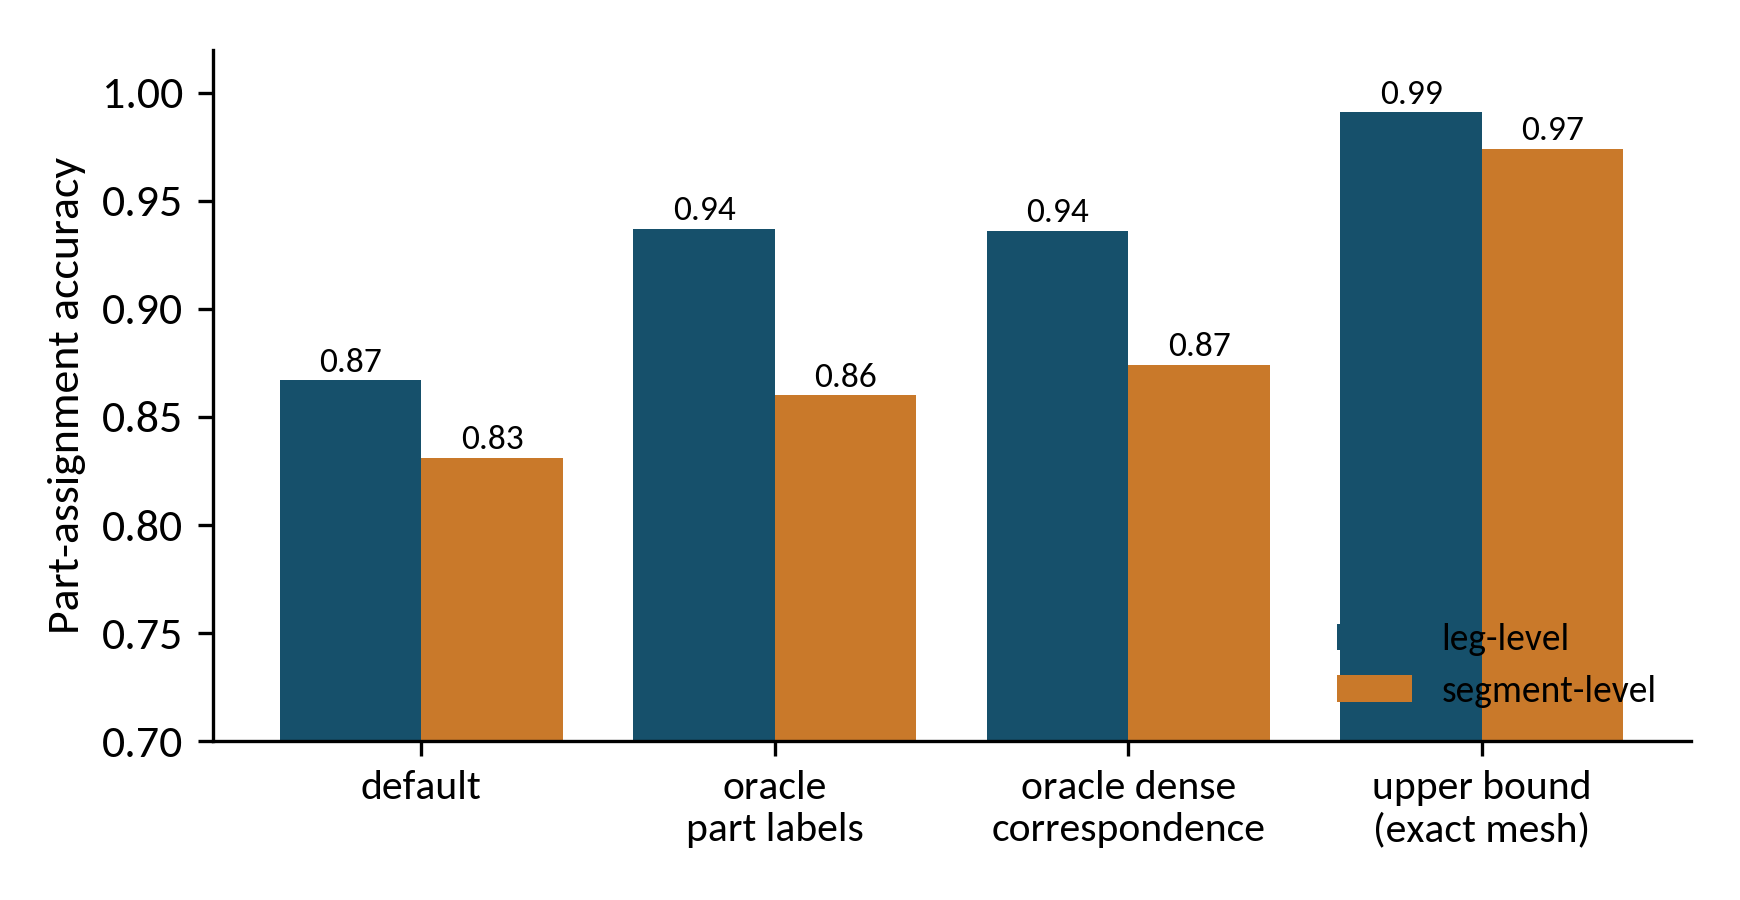
\includegraphics[width=0.46\linewidth]{figures/fig_oracle_ladder.png}
\caption[Oracle ablations]{Part-assignment accuracy on the synthetic benchmark
($n=12$) under oracle part labels and oracle dense correspondence, against the upper
bound of the metric on an exact mesh. Joint-level oracles are evaluated on real
specimens in Section~\ref{sec:skeleton}.}
\label{fig:oracle}
\end{figure}

Supplying the true region of every target point raises accuracy only partially, and
most of the gain comes from a minority of specimens. Supplying exact per-vertex
correspondence improves within-part accuracy on every specimen yet remains clearly
below the upper bound (Figure~\ref{fig:oracle}). Regional identity and within-region
localisation are therefore distinct problems, and correspondence is not the only
missing ingredient: the objective, the optimisation trajectory and the deformation
freedom keep limiting the fit even when correspondence is solved. The oracle that
supplies joint positions is the only one on real data, and it leads into the next
section.
